\documentclass[conference]{IEEEtran}
\IEEEoverridecommandlockouts
% The preceding line is only needed to identify funding in the first footnote. If that is unneeded, please comment it out.
\usepackage{cite}
\usepackage{amsmath,amssymb,amsfonts}
\usepackage{algorithmic}
\usepackage{graphicx}
\usepackage{textcomp}
\usepackage{xcolor}
\usepackage{listings}
\usepackage{url}
\usepackage{booktabs}
\usepackage{float}
\usepackage{array}
\usepackage{tikz}
\usetikzlibrary{shapes.geometric,positioning,arrows.meta}

% Tipos de columna para tablas: texto alineado a la izquierda o centrado.
\newcolumntype{L}[1]{>{\raggedright\arraybackslash}p{#1}}
\newcolumntype{C}[1]{>{\centering\arraybackslash}p{#1}}

\lstset{
	basicstyle=\ttfamily\footnotesize,
	breaklines=true,
	frame=single,
	columns=fullflexible,
	keepspaces=true,
	showstringspaces=false,
	captionpos=b,
	numbers=left,
	numberstyle=\tiny,
	numbersep=4pt
}
\def\BibTeX{{\rm B\kern-.05em{\sc i\kern-.025em b}\kern-.08em
    T\kern-.1667em\lower.7ex\hbox{E}\kern-.125emX}}
\begin{document}

\title{Informe de Laboratorio Unidad II}

\author{\IEEEauthorblockN{1\textsuperscript{st} Sergio David Percy Monge Muñoz}
	\IEEEauthorblockA{\textit{Escuela de Ingeniería Informática} \\
		\textit{Universidad Nacional de Trujillo}\\
		Trujillo, Perú \\
		smonge@unitru.edu.pe}
	\and
	\IEEEauthorblockN{2\textsuperscript{nd} Given Name Surname}
	\IEEEauthorblockA{\textit{dept. name of organization (of Aff.)} \\
		\textit{Universidad Nacional de Trujillo}\\
		Trujillo, Perú \\
		smonge@unitru.edu.pe}
}

\maketitle
%=====================================================================
% SEMANA 6 -- Sistemas basados en el conocimiento
% Plantilla base en formato IEEEtran
% Estructura exigida: Marco Teorico (solo conceptos) + Marco Practico
% Rubrica: que el marco teorico y practico faciliten la comprension
%          al 100% del ejercicio.
%=====================================================================

% Macro auxiliar para marcar los espacios que el autor debe completar.
\providecommand{\TODO}[1]{\textcolor{red}{\textbf{[PENDIENTE: #1]}}}

\section{SEMANA 6: Sistemas Expertos}
\label{sec:semana6}

La presente secci\'on documenta el desarrollo de la sexta semana de
laboratorio, cuyo eje tem\'atico son los \emph{sistemas basados en el
conocimiento} y, en particular, los \emph{sistemas expertos} (SE). El
informe se organiza en dos marcos: el \textbf{marco te\'orico}, que
re\'une exclusivamente los conceptos necesarios para comprender la
soluci\'on, y el \textbf{marco pr\'actico}, que presenta la soluci\'on
de los cuatro ejercicios propuestos. Los ejercicios abarcan la revisi\'on
de la gu\'ia de construcci\'on de un SE, la correcci\'on del diagrama de
dependencias del caso \emph{Analista de Red LAN}, la elaboraci\'on del
programa de dicho caso y la implementaci\'on de un SE de diagn\'ostico
m\'edico r\'apido desplegado en Streamlit.

%=====================================================================
\subsection{Marco Te\'orico}
%=====================================================================

\subsubsection{Sistemas basados en el conocimiento}

Un \textbf{sistema basado en el conocimiento} (SBC, del ingl\'es
\emph{Knowledge-Based System}) es aquel cuyo comportamiento se deriva
principalmente de una representaci\'on expl\'icita de conocimiento sobre
un dominio, y no de un algoritmo fijo codificado l\'inea a l\'inea. La
idea central es la \emph{separaci\'on} entre el conocimiento
(declarativo) y el mecanismo que lo procesa (procedimental), de modo que
el sistema pueda resolver problemas razonando sobre hechos y reglas,
tal como lo har\'ia un especialista humano.

La diferencia esencial frente al software convencional se resume en la
Tabla~\ref{tab:sbc-vs-conv}. En un programa tradicional el conocimiento
est\'a impl\'icito en la l\'ogica de control, mientras que en un SBC
forma un m\'odulo independiente, reutilizable y modificable sin alterar
el motor que razona.

\begin{table}[htbp]
	\caption{Diferencias entre software convencional y sistema basado en el conocimiento}
	\label{tab:sbc-vs-conv}
	\centering
	\small
	\begin{tabular}{p{2.2cm}p{2.6cm}}
		\toprule
		\textbf{Software convencional} & \textbf{Sistema basado en el conocimiento} \\
		\midrule
		El conocimiento est\'a embebido en el c\'odigo. & El conocimiento se representa de forma expl\'icita y separada. \\
		Se modifica reescribiendo el algoritmo. & Se modifica a\~nadiendo o editando reglas/hechos. \\
		No explica el razonamiento. & Puede justificar sus conclusiones. \\
		\bottomrule
	\end{tabular}
\end{table}

\subsubsection{Sistemas expertos}

Un \textbf{sistema experto} es un SBC que emula la capacidad de
razonamiento de un experto humano dentro de un dominio acotado y
espec\'ifico. Sus rasgos caracter\'isticos son: (i) conocimiento
especializado de alta calidad, (ii) razonamiento simb\'olico basado en
reglas o hechos, (iii) capacidad de explicar c\'omo y por qu\'e lleg\'o
a una conclusi\'on, y (iv) la posibilidad de operar con informaci\'on
incompleta o incierta. Entre sus limitaciones destacan la dependencia
de la calidad del conocimiento introducido, la dificultad de abarcar
dominios muy amplios y la incapacidad de aprender por s\'i mismos sin
t\'ecnicas adicionales de aprendizaje autom\'atico.

\subsubsection{Arquitectura de un sistema experto}

Los componentes cl\'asicos de un SE se describen en la
Tabla~\ref{tab:componentes}. La interacci\'on entre ellos constituye el
ciclo de razonamiento: el usuario introduce hechos, el motor de
inferencia los contrasta con las reglas de la base de conocimiento y
genera nuevas conclusiones que se almacenan en la base de hechos.

\begin{table}[htbp]
	\caption{Componentes de un sistema experto}
	\label{tab:componentes}
	\centering
	\small
	\begin{tabular}{p{2.4cm}p{4.2cm}}
		\toprule
		\textbf{Componente} & \textbf{Funci\'on} \\
		\midrule
		Base de conocimiento (BC) & Almacena las reglas y hechos del dominio. \\
		Base de hechos (memoria de trabajo) & Contiene los hechos actuales sobre el caso. \\
		Motor de inferencia (MI) & Aplica las reglas para derivar nuevos hechos. \\
		Interfaz de usuario & Permite al usuario introducir datos y consultar resultados. \\
		Subsistema de explicaci\'on & Justifica las conclusiones alcanzadas. \\
		Adquisici\'on del conocimiento & Permite al ingeniero del conocimiento introducir y depurar reglas. \\
		\bottomrule
	\end{tabular}
\end{table}

\subsubsection{Representaci\'on del conocimiento mediante reglas de producci\'on}

El formalismo m\'as difundido es la \textbf{regla de producci\'on},
expresada como una implicaci\'on l\'ogica:

\begin{center}
	\texttt{SI} $\langle$condiciones$\rangle$ \texttt{ENTONCES}
	$\langle$acci\'on o conclusi\'on$\rangle$.
	\label{eq:regla}
\end{center}

La parte izquierda se denomina \emph{antecedente} o premisa y la derecha
\emph{consecuente} o acci\'on. Cuando el antecedente se satisface con los
hechos de la memoria de trabajo, la regla se \emph{dispara} y su
consecuente se agrega como un nuevo hecho. Para tratar informaci\'on
incompleta se emplean los \textbf{factores de certeza} (FC, del ingl\'es
\emph{Certainty Factor}), valores en el rango $[-1,1]$ que cuantifican el
grado de confianza en un hecho o regla.

\subsubsection{Motor de inferencia y estrategias de encadenamiento}

El motor de inferencia recorre iterativamente tres pasos:
\emph{reconocimiento} (identificar las reglas aplicables),
\emph{selecci\'on} (resolver conflictos cuando varias reglas compiten) y
\emph{acci\'on} (disparar la regla elegida). Existen dos estrategias de
razonamiento, comparadas en la Tabla~\ref{tab:encadenamiento}.

\begin{table}[htbp]
	\caption{Estrategias de encadenamiento del motor de inferencia}
	\label{tab:encadenamiento}
	\centering
	\small
	\begin{tabular}{p{1.9cm}p{2.4cm}p{2.4cm}}
		\toprule
		& \textbf{Hacia adelante} & \textbf{Hacia atr\'as} \\
		\midrule
		Direcci\'on & De los datos a las conclusiones. & De la hip\'otesis a los datos. \\
		Aplicaci\'on & Diagn\'ostico, monitorizaci\'on. & Conjetura y verificaci\'on. \\
		Inicio & Hechos observados. & Conclusi\'on por demostrar. \\
		\bottomrule
	\end{tabular}
\end{table}

\subsubsection{Metodolog\'ia para construir un sistema experto}

La construcci\'on de un SE sigue, en general, las fases de la
Tabla~\ref{tab:fases}. Este es el eje de la gu\'ia revisada en el
Ejercicio~1. La actividad del \textbf{ingeniero del conocimiento}
consiste en extraer el conocimiento del experto humano
(\emph{adquisici\'on}), representarlo formalmente y validarlo.

\begin{table}[htbp]
	\caption{Fases de la metodolog\'ia de construcci\'on de un sistema experto}
	\label{tab:fases}
	\centering
	\small
	\begin{tabular}{p{2.1cm}p{4.4cm}}
		\toprule
		\textbf{Fase} & \textbf{Actividad principal} \\
		\midrule
		Identificaci\'on & Definir el problema, el alcance y los expertos. \\
		Conceptualizaci\'on & Organizar conceptos, variables y relaciones del dominio. \\
		Formalizaci\'on & Representar el conocimiento (reglas, hechos, incertidumbre). \\
		Implementaci\'on & Codificar la BC y el MI en una herramienta o lenguaje. \\
		Validaci\'on & Contrastar las respuestas con el experto humano. \\
		Mantenimiento & Ampliar y corregir la base de conocimiento. \\
		\bottomrule
	\end{tabular}
\end{table}

\subsubsection{Herramientas de implementaci\'on}

Un SE puede implementarse con lenguajes y entornos diversos. Los
lenguajes simb\'olicos como \textbf{Prolog} y \textbf{CLIPS} ofrecen
motores de inferencia nativos; en el ecosistema de \textbf{Python}
pueden emplearse bibliotecas de reglas (por ejemplo, \texttt{experta} o
\texttt{durable-rules}) combinadas con \textbf{Streamlit} para construir
interfaces web interactivas de forma r\'apida. Streamlit permite exponer
el SE como una aplicaci\'on accesible desde el navegador, recalculando
las conclusiones cada vez que el usuario modifica los s\'intomas o
hechos de entrada.

%=====================================================================
\subsection{Marco Pr\'actico}
%=====================================================================

En este marco se resuelven los cuatro ejercicios propuestos para la
semana. Cada subsecci\'on incluye la descripci\'on de la actividad, los
resultados obtenidos y las evidencias correspondientes.

\subsubsection{Ejercicio 1: Revisi\'on de la gu\'ia para construir un Sistema Experto}

\textbf{Objetivo.} Revisar y sintetizar la gu\'ia de construcci\'on de
un SE, identificando cada fase y su producto entregable.

\textbf{Desarrollo.} \TODO{Resumir con sus propias palabras la gu\'ia
revisada y completar la Tabla~\ref{tab:guia} relacionando cada fase con
la actividad realizada y su entregable.}

\begin{table}[htbp]
	\caption{S\'intesis de la gu\'ia de construcci\'on de un SE}
	\label{tab:guia}
	\centering
	\small
	\begin{tabular}{p{1.9cm}p{2.6cm}p{2.0cm}}
		\toprule
		\textbf{Fase} & \textbf{Actividad} & \textbf{Entregable} \\
		\midrule
		Identificaci\'on & \TODO{} & \TODO{} \\
		Conceptualizaci\'on & \TODO{} & \TODO{} \\
		Formalizaci\'on & \TODO{} & \TODO{} \\
		Implementaci\'on & \TODO{} & \TODO{} \\
		Validaci\'on & \TODO{} & \TODO{} \\
		Mantenimiento & \TODO{} & \TODO{} \\
		\bottomrule
	\end{tabular}
\end{table}

\subsubsection{Ejercicio 2: Caso Analista de Red LAN -- correcci\'on del diagrama de dependencias}

\textbf{Objetivo.} Revisar el caso del \emph{Analista de Red LAN} y
corregir el diagrama de dependencias asociado al problema.

\textbf{Descripci\'on del caso.} El caso modela el razonamiento de un
analista que diagnostica fallas en una red de \'area local (LAN) a
partir de s\'intomas observables. El dominio se representa mediante
variables y relaciones de dependencia entre ellas, que constituir\'an
la base de conocimiento del sistema experto.

\textbf{Correcci\'on realizada.} \TODO{Describir los errores encontrados
en el diagrama original (flechas invertidas, nodos faltantes,
relaciones redundantes o dependencias mal jerarquizadas) y c\'omo se
corrigieron. El diagrama corregido se muestra en la
Fig.~\ref{fig:analista-lan}, dentro del Ejercicio~3.}

\begin{table}[htbp]
	\caption{Variables y dependencias del caso Analista de Red LAN}
	\label{tab:lan}
	\centering
	\small
	\begin{tabular}{p{2.4cm}p{2.4cm}p{1.7cm}}
		\toprule
		\textbf{Variable} & \textbf{Depende de} & \textbf{Tipo} \\
		\midrule
		\TODO{} & \TODO{} & \TODO{} \\
		\TODO{} & \TODO{} & \TODO{} \\
		\TODO{} & \TODO{} & \TODO{} \\
		\bottomrule
	\end{tabular}
\end{table}

\subsubsection{Ejercicio 3: Programa del caso Analista de Red LAN}

\textbf{Objetivo.} Elaborar el programa que implementa el sistema experto
del caso \emph{Analista de Red LAN}, tomando como base el diagrama de
dependencias corregido.

\textbf{Diagrama de dependencias.} La Fig.~\ref{fig:analista-lan}
presenta el diagrama de dependencias utilizado por el programa para
encadenar los s\'intomas hacia las posibles causas de falla.

\begin{figure}[H]
	\centering
	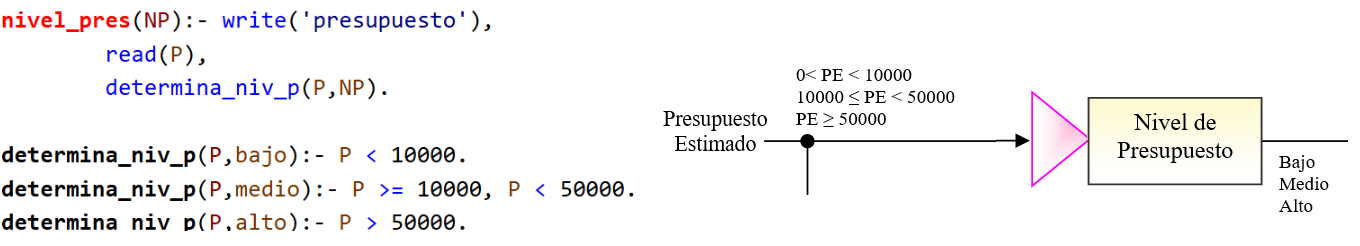
\includegraphics[width=\linewidth]{images/semana_6/3_analista-lan.png}
	\caption{Diagrama de dependencias del caso Analista de Red LAN empleado por el programa.}
	\label{fig:analista-lan}
\end{figure}

\textbf{Dise\~no de la base de conocimiento.} \TODO{Enumerar las reglas
de producci\'on del caso (s\'intoma $\rightarrow$ causa). Puede usarse
la estructura \texttt{SI ... ENTONCES ...} y los factores de certeza si
el caso lo requiere.}

\textbf{Implementaci\'on.} El programa aplica encadenamiento hacia
adelante sobre los hechos introducidos por el usuario. El
Listado~\ref{lst:analista-lan} muestra la estructura general del c\'odigo.

\begin{lstlisting}[language=Python,caption={Estructura del programa del caso Analista de Red LAN},label={lst:analista-lan}]
# Base de conocimiento: lista de reglas (sintoma -> causa)
REGLAS = [
    # TODO: completar con las reglas del diagrama de dependencias
]

def motor_inferencia(hechos):
    """Aplica encadenamiento hacia adelante hasta estabilizar."""
    nueva = True
    while nueva:
        nueva = False
        for regla in REGLAS:
            if regla.condicion(hechos) and regla.conclusion not in hechos:
                hechos.append(regla.conclusion)
                nueva = True
    return hechos

if __name__ == "__main__":
    # TODO: interfaz / prueba del sistema
    pass
\end{lstlisting}

\subsubsection{Ejercicio 4: Sistema experto para el diagn\'ostico r\'apido de una enfermedad}

\textbf{Objetivo.} Implementar un SE de diagn\'ostico r\'apido de una
enfermedad, delimitado a una \'unica especialidad de la salud, y
desplegarlo como aplicaci\'on en Streamlit.

\textbf{Delimitaci\'on del dominio.} Especialidad elegida:
\TODO{indicar la especialidad (por ejemplo, cardiolog\'ia,
endocrinolog\'ia, dermatolog\'ia, etc.) y el conjunto acotado de
enfermedades que el sistema podr\'a identificar.}

\textbf{Base de conocimiento.} La Tabla~\ref{tab:medicina} relaciona
s\'intomas con posibles diagn\'osticos dentro de la especialidad
elegida.

\begin{table}[htbp]
	\caption{Reglas del sistema experto de diagn\'ostico m\'edico}
	\label{tab:medicina}
	\centering
	\small
	\begin{tabular}{p{2.7cm}p{2.2cm}p{1.7cm}}
		\toprule
		\textbf{S\'intomas (SI)} & \textbf{Diagn\'ostico (ENTONCES)} & \textbf{FC} \\
		\midrule
		\TODO{} & \TODO{} & \TODO{} \\
		\TODO{} & \TODO{} & \TODO{} \\
		\TODO{} & \TODO{} & \TODO{} \\
		\bottomrule
	\end{tabular}
\end{table}

\textbf{Implementaci\'on en Streamlit.} \TODO{Describir la arquitectura
de la aplicaci\'on (entradas del usuario, motor de inferencia, salida
del diagn\'ostico y mensaje de recomendaci\'on de consultar a un
especialista).}

\textbf{Enlace de la soluci\'on.} Aplicaci\'on desplegada:

\begin{center}
	\url{\TODO{https://...streamlit.app}}
\end{center}

%=====================================================================
\subsection{S\'intesis de la semana}
%=====================================================================

\TODO{Redactar una s\'intesis breve que conecte el marco te\'orico con
los cuatro ejercicios resueltos y se\~nale las lecciones aprendidas.}

\section{Semana 7}

\section{Semana 8}

\section{Semana 9}

\section{Conclusiones}


\end{document}

